\documentclass{ctexbeamer}
\setbeamercolor{titlelike}{parent=structure,bg=lightgray}
\setbeamercovered{transparent}
\usefonttheme{structurebold}
\usetheme{CambridgeUS}
%\usecolortheme{rose}
%\usecolortheme{beaver}
\usecolortheme{crane}
\useoutertheme{infolines}

\usepackage{hyperref} 
\usepackage[backend=biber,style=authortitle]{biblatex}
%\usepackage[backend=bibtex,sorting=none]{biblatex}
%\addbibresource{main.bib}
%\setbeamerfont{footnote}{size=\tiny}
\usepackage{datetime}

\newdateformat{monthyeardate}{%
      \THEYEAR.\THEMONTH}

\renewcommand{\figurename}{Fig}


\title{ISAIC2020: Privacy Enhancement for Vehicle's Long Term Credential in V2X using Direct Anonymous Attestation}

\author{Pan Lanlan (潘蓝兰) \newline  \newline abbypan@gmail.com} 
\institute[China]{Guangdong OPPO Mobile Telecommunications Corp. Ltd., China} 

\date{\monthyeardate\today}

\begin{document}

\frame{\titlepage}

\frame{\tableofcontents}
\clearpage

\section{Background}

\subsection{Connected Car}
\begin{frame}
\frametitle{Connected Car}

    \url{https://www.qorvo.com/design-hub/blog/v2x-in-the-connected-car-of-the-future}

    \begin{figure}[H]
        \centering 
        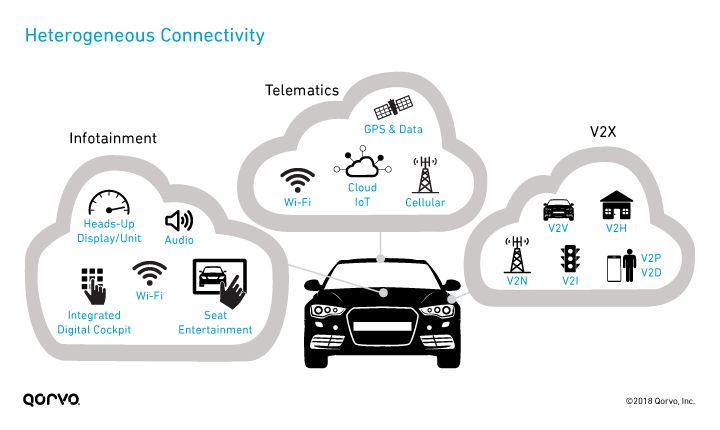
\includegraphics[width=0.7\textwidth]{pic/connectivity.png} 
        \caption{Connectivity} 
        \label{fig.connectivity}
    \end{figure}

\end{frame}

\subsection{V2X Communication}
\begin{frame}
\frametitle{V2X Communication}

    \url{https://www.researchgate.net/publication/331676083_Software-Defined_Heterogeneous_Vehicular_Networking_The_Architectural_Design_and_Open_Challenges/}

    \begin{figure}[H]
        \centering 
        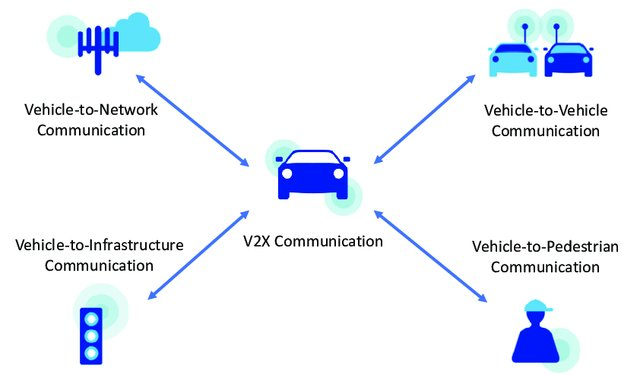
\includegraphics[width=0.7\textwidth]{pic/v2x.jpg} 
        \caption{V2X Communication} 
        \label{fig.v2x}
    \end{figure}

\end{frame}

\subsection{Personally Identifiable Information (PII)}
\begin{frame}
\frametitle{Personally Identifiable Information (PII)}

Avoid tracking.

GDPR: Prevent attackers or insiders from collecting Personally Identifiable Information (PII).

    \url{https://cyberscout.com/nl/blog/recipe-for-a-safer-identity-is-as-easy-as-pii}

    \begin{figure}[H]
        \centering 
        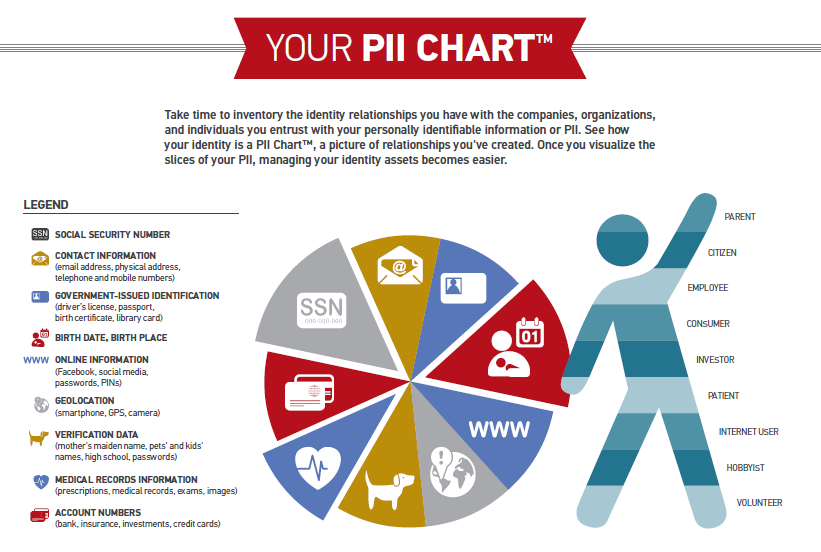
\includegraphics[width=0.6\textwidth]{pic/pii.png} 
        \caption{PII} 
        \label{fig.pii}
    \end{figure}

\end{frame}

\subsection{Privacy in V2X Communication}
\begin{frame}
\frametitle{Privacy in V2X Communication}

    \begin{itemize}
            \item Confidential
            \item Anonymous
            \item Pseudonymous
            \item Conditional Traceable, Protect PII
        \end{itemize}

\end{frame}

\section{Related Work}

\subsection{Direct Anonymous Attestation (DAA) Scheme}
\begin{frame}
\frametitle{Direct Anonymous Attestation (DAA) Scheme}

    \url{https://www.researchgate.net/publication/225162761_On_a_Possible_Privacy_Flaw_in_Direct_Anonymous_Attestation_DAA}

    \begin{figure}[H]
        \centering 
        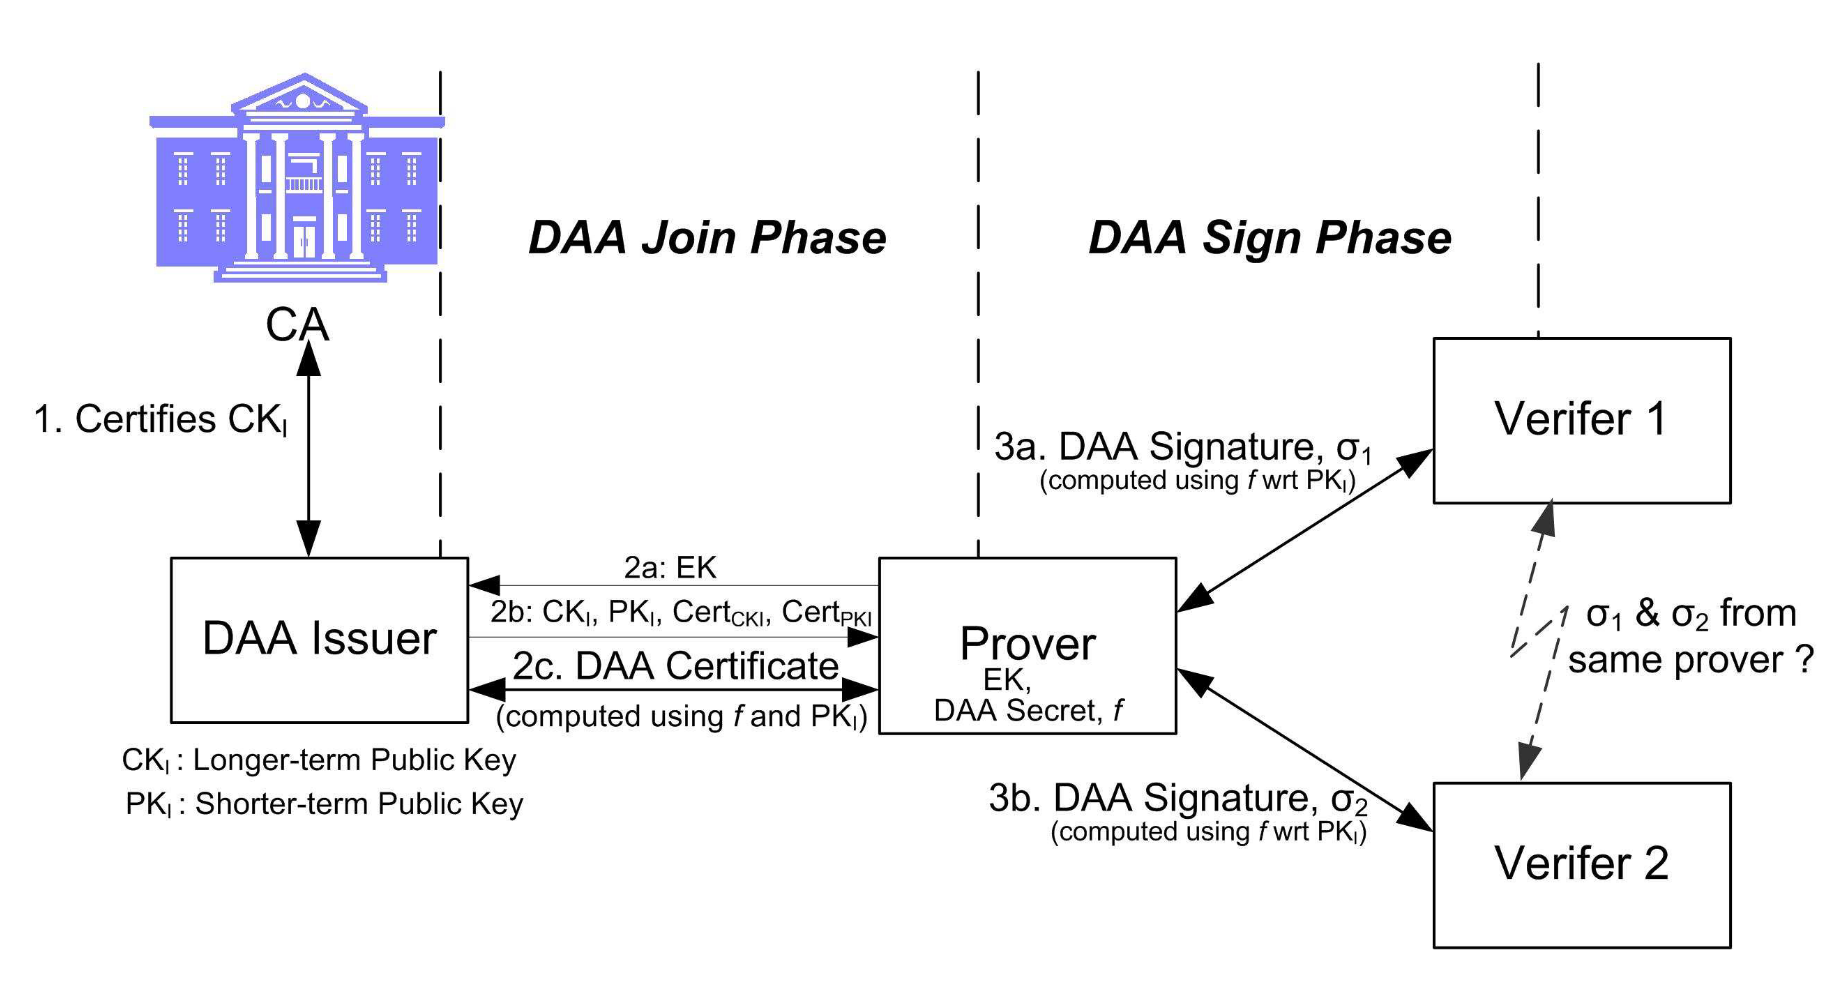
\includegraphics[width=0.8\textwidth]{pic/daa.png} 
        \caption{DAA} 
        \label{fig.daa}
    \end{figure}
\end{frame}

\subsection{V2X DAA}
\begin{frame}
\frametitle{Privacy-Enhanced Capabilities for VANETs using Direct Anonymous Attestation}

    \url{https://www.researchgate.net/publication/321422009_Privacy-Enhanced_Capabilities_for_VANETs_using_Direct_Anonymous_Attestation}

    \begin{figure}[htbp]
        \centering
        \begin{minipage}[t]{0.48\textwidth}
            \centering
            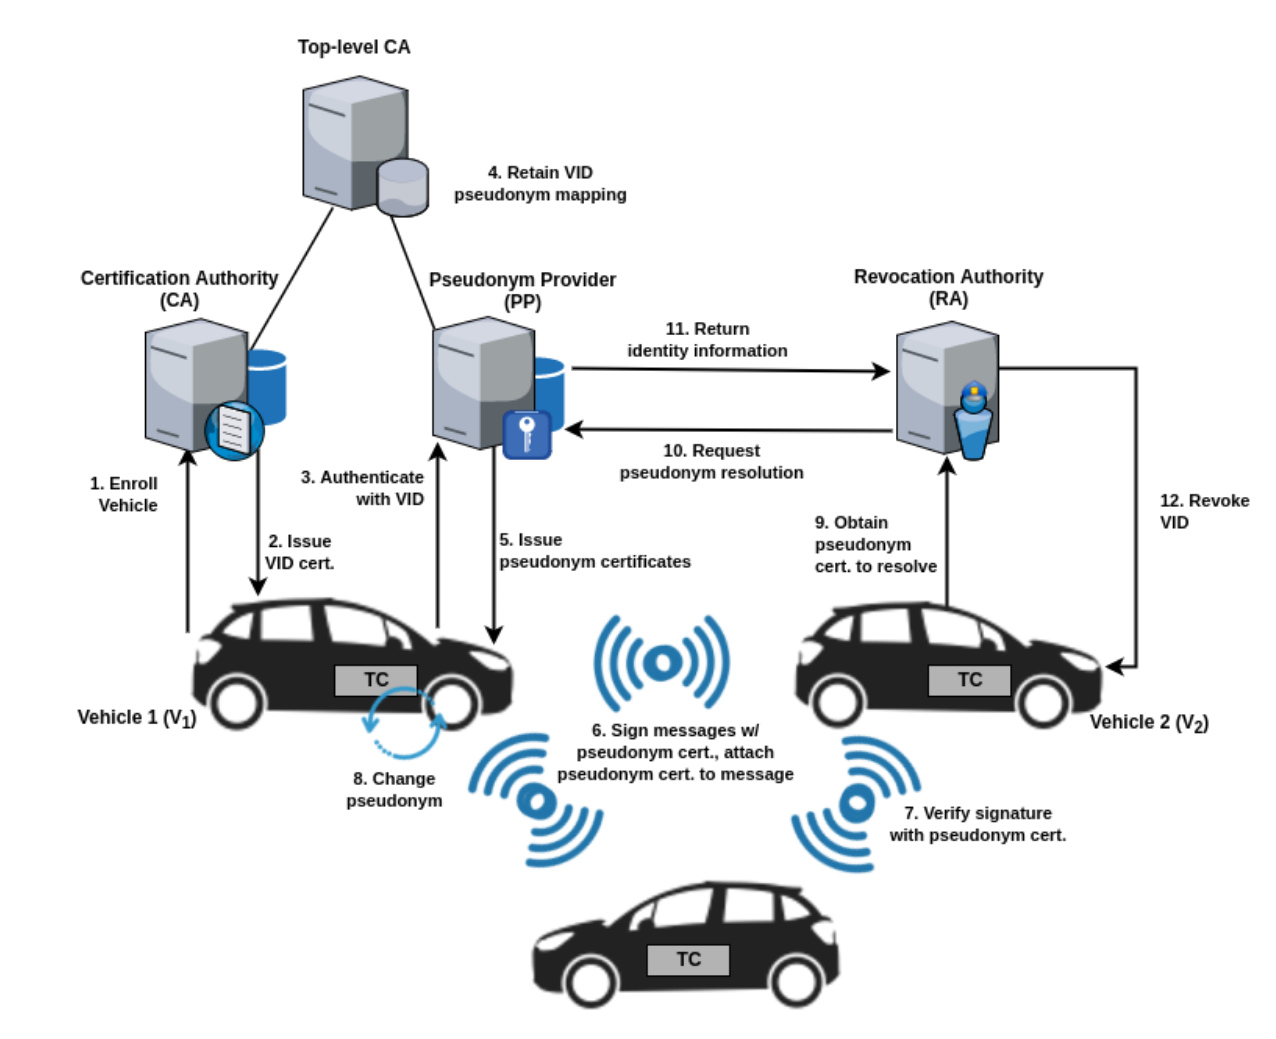
\includegraphics[width=0.9\textwidth]{pic/v2x.pki.png}
           \caption{V2X PKI}
        \end{minipage}
        \begin{minipage}[t]{0.48\textwidth}
            \centering
            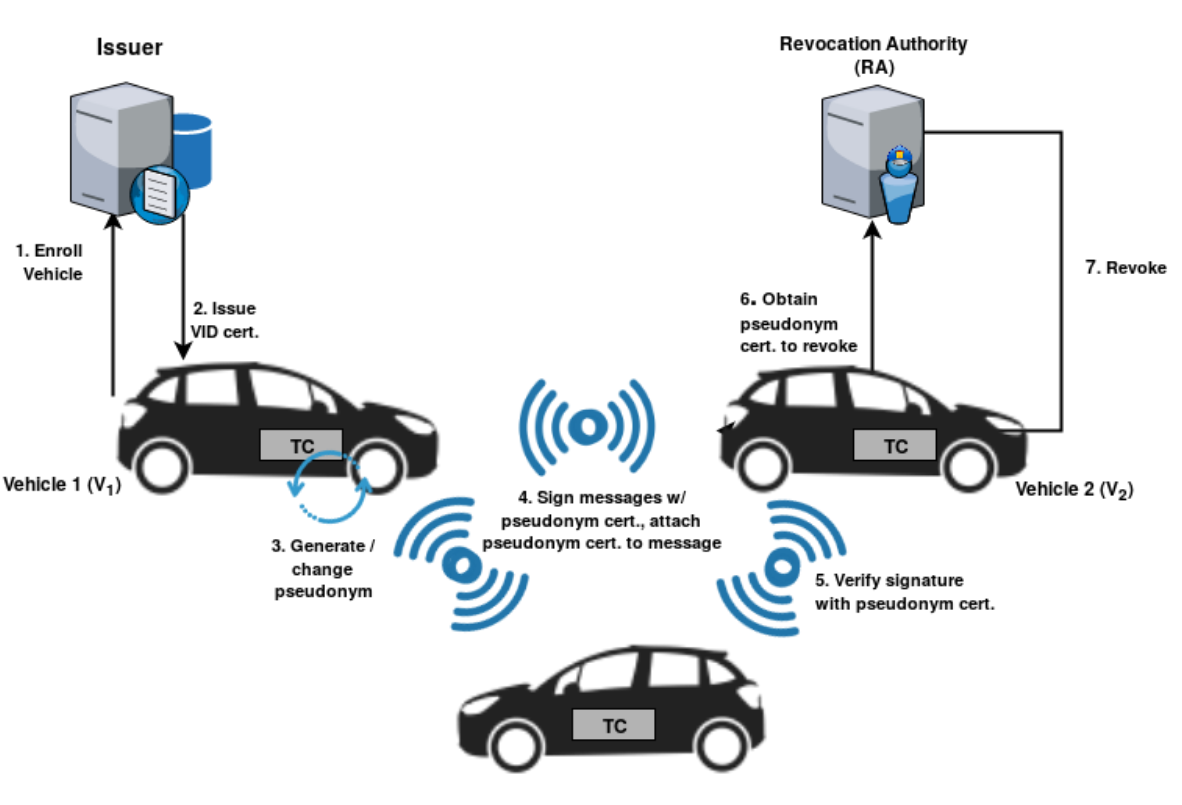
\includegraphics[width=0.9\textwidth]{pic/v2x.daa.png}
            \caption{V2X DAA}
        \end{minipage}
    \end{figure}

\end{frame}

\begin{frame}
%\frametitle{Privacy-Enhanced Capabilities for VANETs using Direct Anonymous Attestation}

    \begin{figure}[H]
        \centering 
        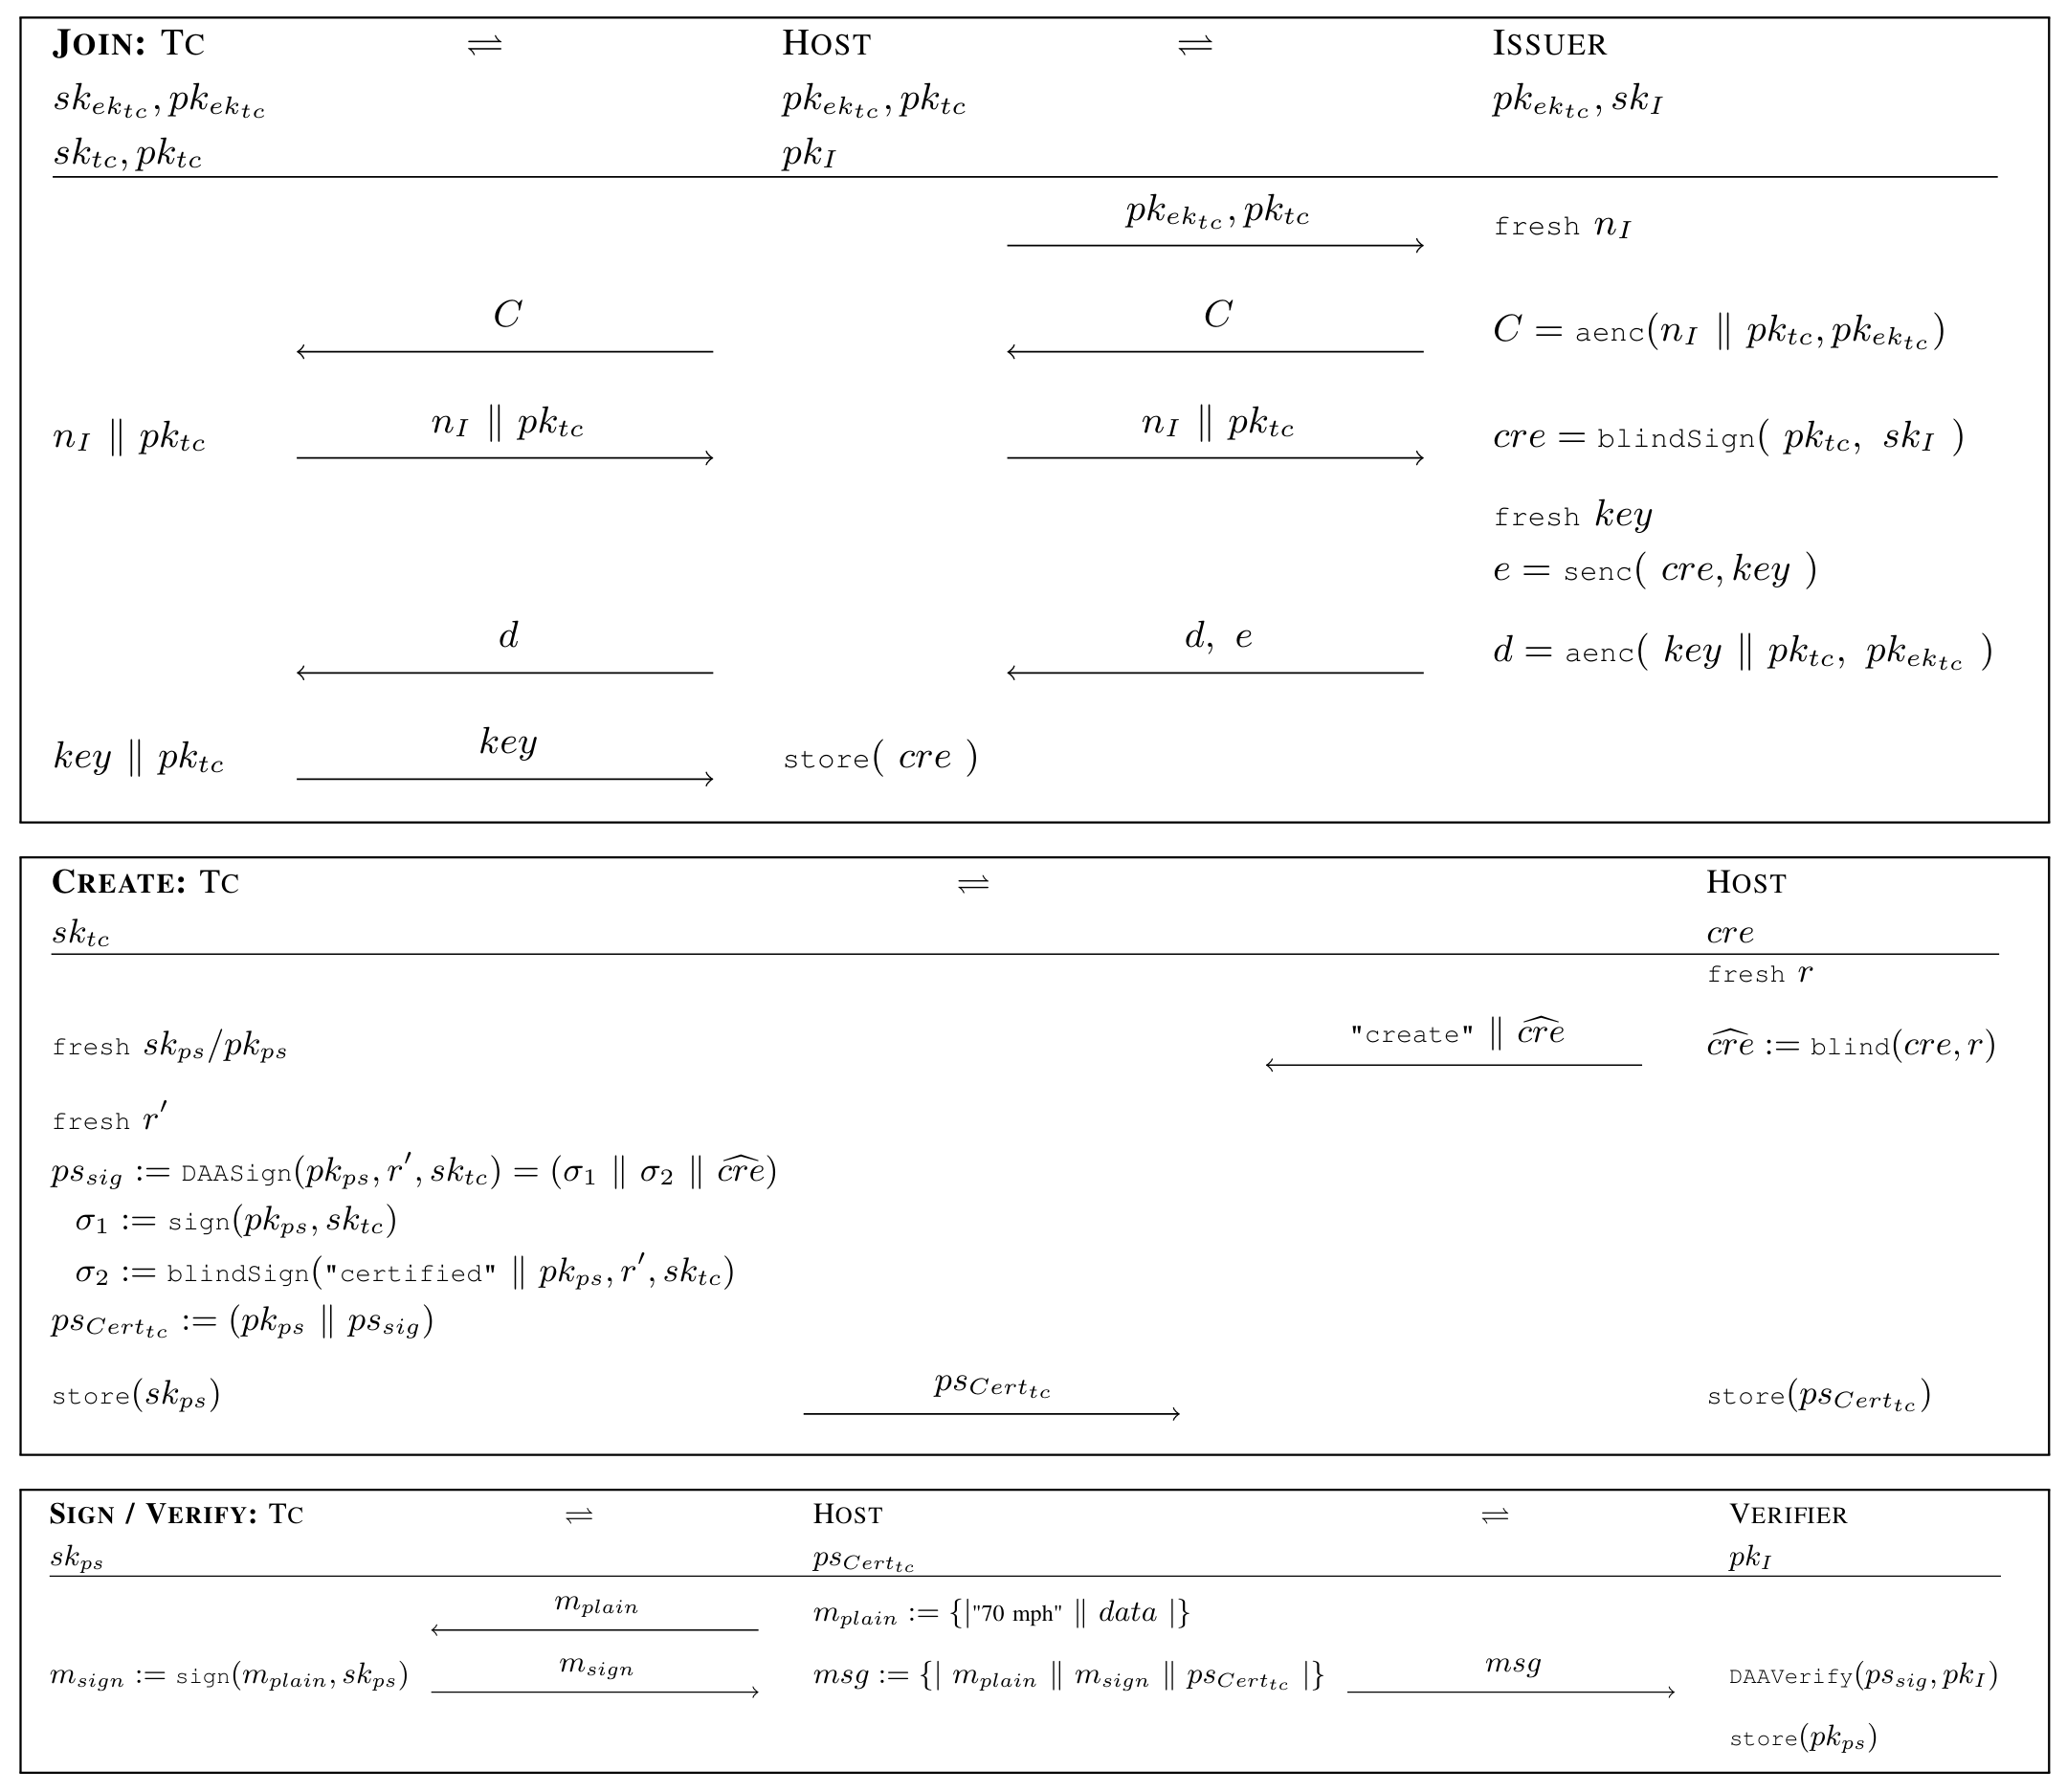
\includegraphics[width=0.75\textwidth]{pic/v2x.daa.crypto.png} 
        \caption{V2X DAA protocol} 
        \label{fig.v2x.daa.crypto}
    \end{figure}

\end{frame}


\begin{frame}
\frametitle{Securing V2X Communications for the Future}

    \url{https://www.researchgate.net/publication/335089342_Securing_V2X_Communications_for_the_Future_Can_PKI_Systems_offer_the_answer}

    \begin{figure}[htbp]
        \centering
        \begin{minipage}[t]{0.48\textwidth}
            \centering
            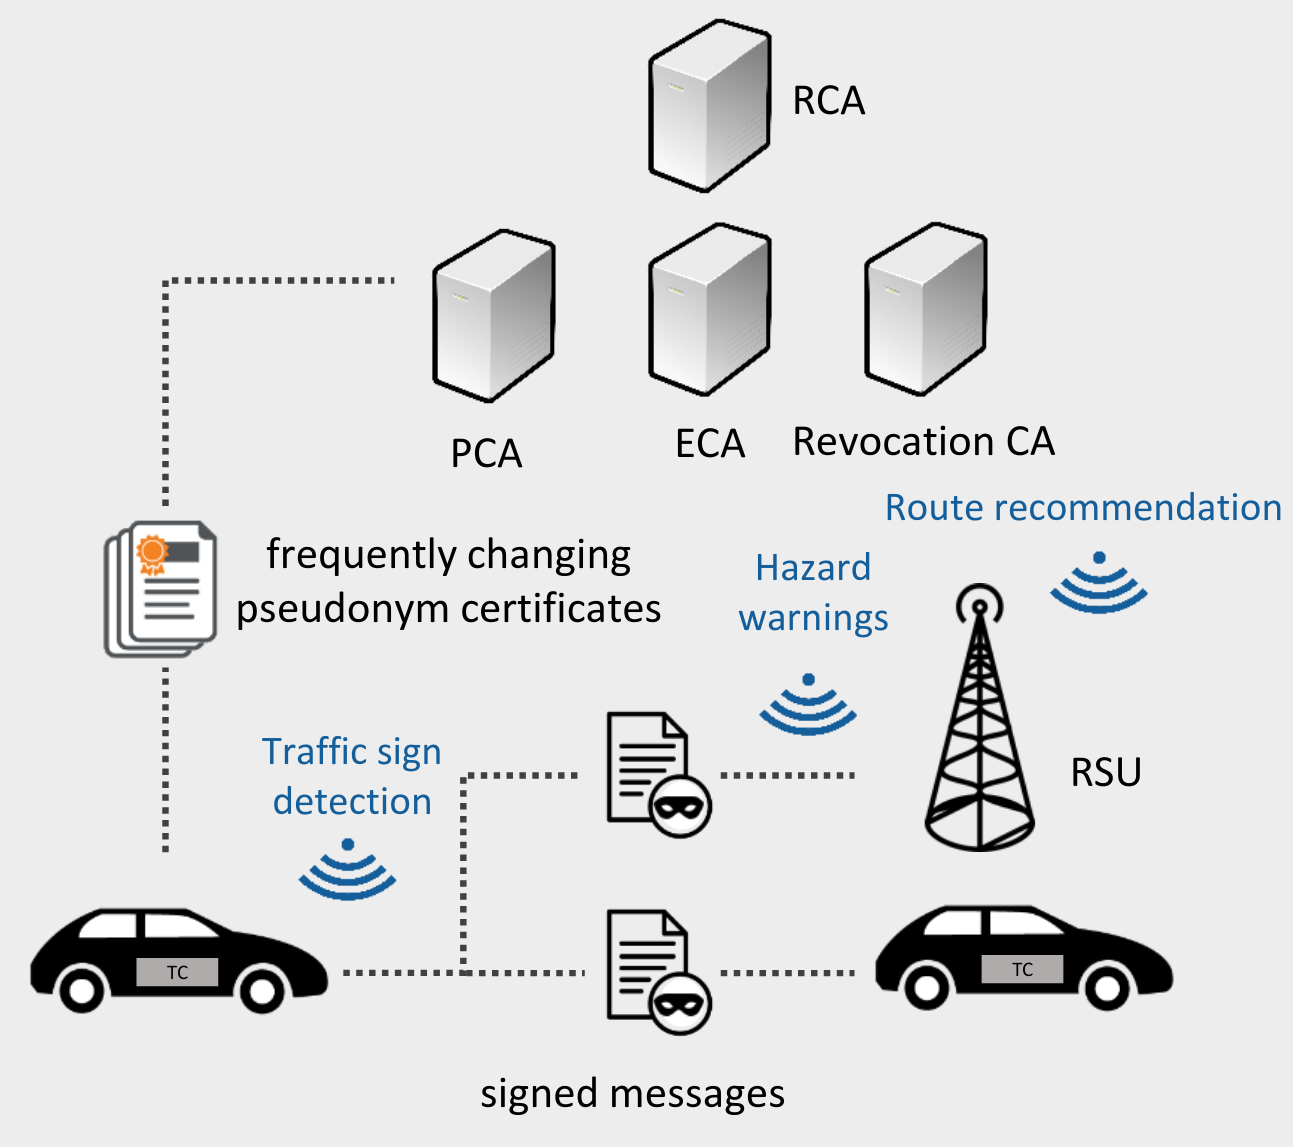
\includegraphics[width=0.9\textwidth]{pic/v2x.pki2.png}
           \caption{V2X PKI}
        \end{minipage}
        \begin{minipage}[t]{0.48\textwidth}
            \centering
            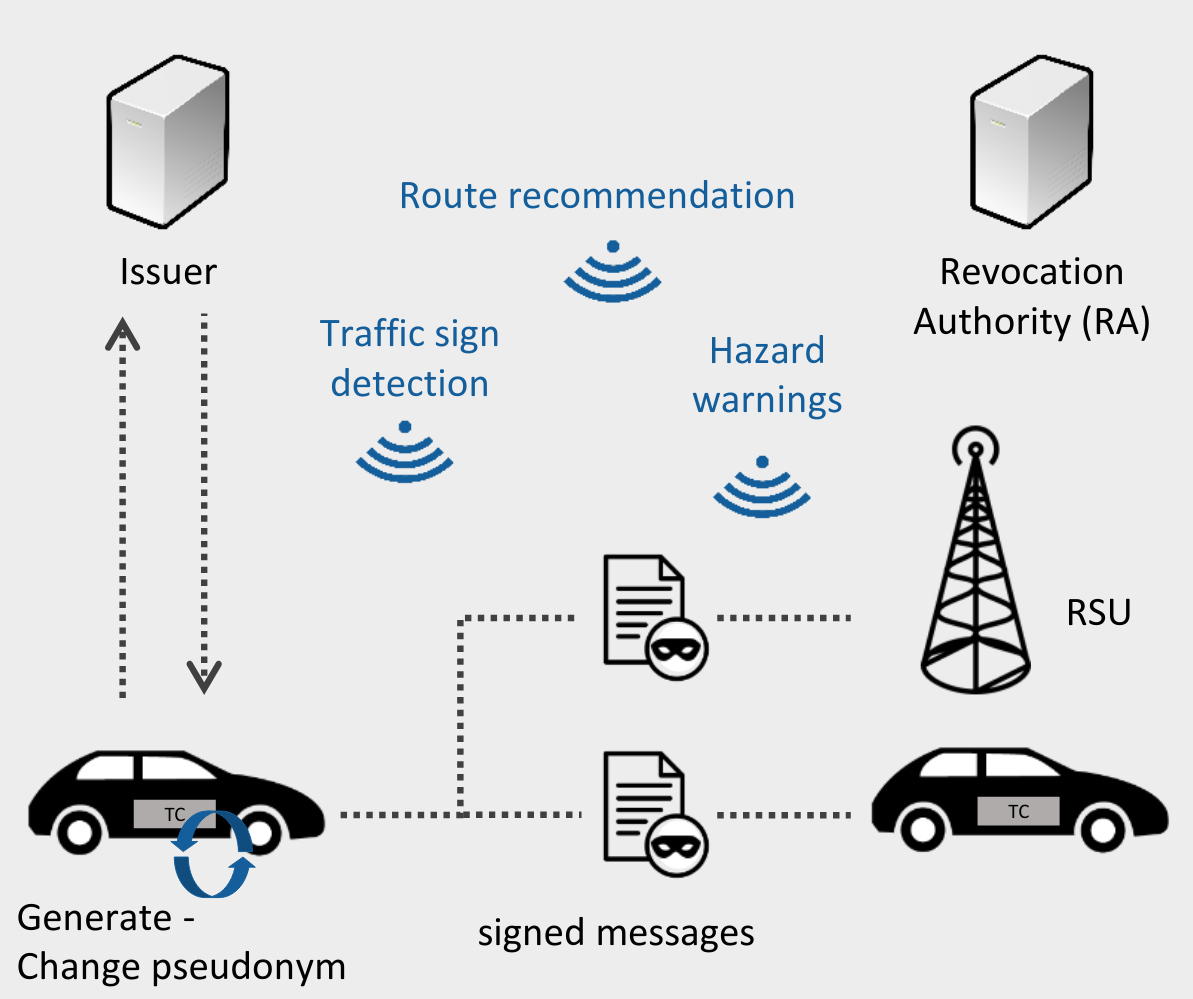
\includegraphics[width=0.9\textwidth]{pic/v2x.daa2.png}
            \caption{V2X DAA}
        \end{minipage}
    \end{figure}

\end{frame}

\subsection{Problem}
\begin{frame}
\frametitle{Problem}

Traditional VID Certificate is a long-term credential, it is traceable by Pseudonymous CA. 
\newline
Therefore, it is hard to scale if we want to enhance the privacy protection from Pseudonymous CA insiders.
\newline
\newline

Above DAA schemes make the enrollment authority write long-term pseudonymous certificate into vehicle, remove short-term pseudonymous certificate.
\newline
It is simpler than traditional V2X solution.
However, the trust is mostly shift to vehicle.

\end{frame}

\section{Our Proposal}

\subsection{Overview}
\begin{frame}
\frametitle{Privacy Enhancement for Vehicle's Long Term Credential in V2X using Direct Anonymous Attestation}

Enrollment authority writes long-term pseudonymous credential into vehicle.
\newline
Reserve the Pseudonymous Authority to issue short-term pseudonymous credential for vehicle.

    \begin{figure}[H]
        \centering 
        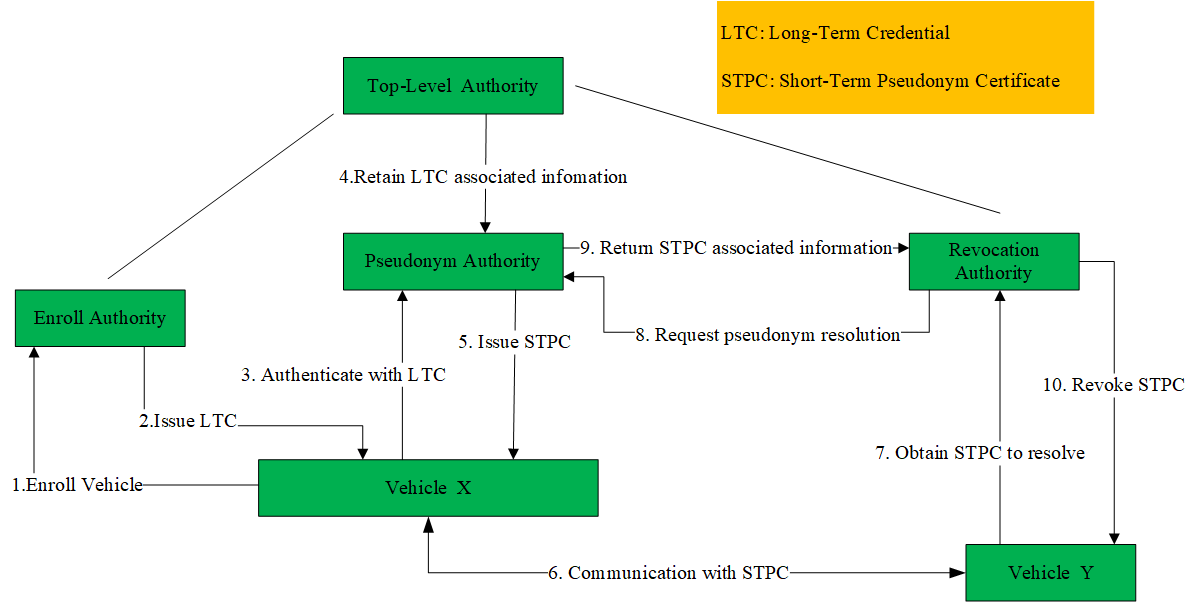
\includegraphics[width=0.70\textwidth]{pic/ltc.daa.png} 
        \caption{DAA: Long Term Credential} 
        \label{fig.ltc.daa}
    \end{figure}

\end{frame}

\subsection{Issue Short-Term Pseudonymous Certificate}
\begin{frame}
\frametitle{Issue Short-Term Pseudonymous Certificate}

Vehicle’s long-term pseudonymous credential is used to authenticate the request for short-term pseudonymous credential.
\newline
\newline
The verifier is Pseudonymous Authority.

    \begin{figure}[H]
        \centering 
        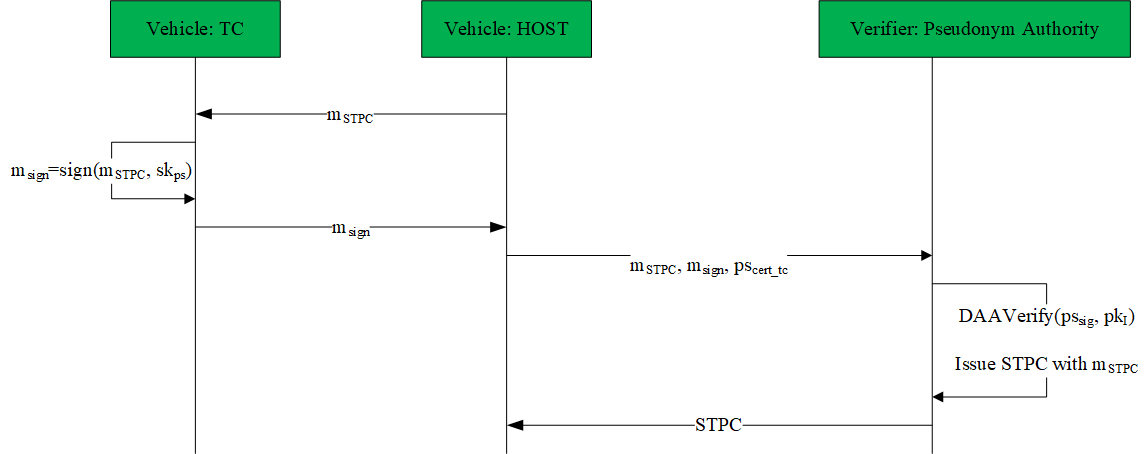
\includegraphics[width=0.75\textwidth]{pic/ltc.detail.png} 
        \caption{Issue Short-Term Pseudonymous Certificate} 
        \label{fig.ltc.detail}
    \end{figure}
\end{frame}

\subsection{Conclusion}
\begin{frame}
\frametitle{Conclusion}

Privacy enhancement is critical for person in V2X scenario.
\newline
\newline
We should build up the future V2X ecosystem with the principles of 'privacy by design' and 'privacy by default'.
\newline
\newline

\end{frame}

%\subsection{Resources}
%\begin{frame}{Resources}

    %\begin{thebibliography}{99}
        %\bibitem{rtlwifi} RTLWIFI
            %https://arstechnica.com/information-technology/2019/10/unpatched-linux-flaw-may-let-attackers-crash-or-compromise-nearby-devices/
    %\end{thebibliography}

%\end{frame}

\end{document}
